\section {Benutzer und Gruppen}

In GNU/Linux gibt es -- wie in allen unixoiden Betriebssystemen -- verschiedene Benutzer. Damit sind nicht nur einzelne Zugänge für Personen, die den Computer verwenden, gemeint. Für viele Systemdienste (z.B. Druckerdienste) wird automatisch ein eigener Benutzer mit bestimmten Berechtigungen angelegt. Zusätzlich zu den Benutzern gibt es verschiedene Benutzergruppen. Sowohl für Benutzer als auch für Gruppen lassen sich unterschiedliche Berechtigungen festlegen. Dadurch wird erreicht, dass eine mögliche Schwachstelle in einem Dienst nicht zu große Auswirkungen auf das System haben kann.  

\subsection {sudo}
Jeder ``menschliche'' Benutzer hat jeweils ein eigenes Benutzerverzeichnis in \lstinline|/home|. Unter normalen Bedingungen hat jeder ``normale'' Benutzer nur in seinem eigenen home--Verzeichnis Schreibrechte. D.h. er kann keine Programme installieren oder sonstige Änderungen am System vornehmen. Für alle diese Aufgaben ist unter GNU/Linux traditionell der Benutzer \lstinline|root| zuständig. \footnote{\lstinline|root| bezeichnet also einerseits die Wurzel des Dateisystems, andererseits den ``Administrator''.} Bei modernen Systemen wie Ubuntu oder Debian kann man sich aber nicht direkt als \lstinline|root| anmelden. Stattdessen können normale Benutzer (mit den entsprechenden Berechtigungen) mit Hilfe des Befehls \lstinline|sudo| temporär in die Rolle von \lstinline|root| schlüpfen. Dazu wird einfach der Befehl \lstinline|sudo| vor den eigentlichen Befehl gestellt. Bevor der Befehl ausgeführt wird, wird man nach seinem Passwort gefragt. Man erhält dabei keine Ausgabe, man muss das Passwort also ``blind'' eingeben.

\begin{lstlisting}
bob@computer:~$ mkdir /folder
mkdir: das Verzeichnis "/folder" kann nicht angelegt werden: Keine Berechtigung
bob@computer:~$ sudo mkdir /folder
[sudo] Passwort für bob: 
bob@computer:~$ 
\end{lstlisting}

\begin{figure}[H]
 \begin{center}
  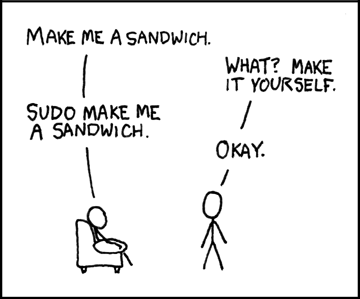
\includegraphics[width=6cm,keepaspectratio=true]{sudo.png}
  \caption{Quelle: \url{http://www.xkcd.com}}
 \end{center}
\end{figure}

\subsection {Benutzerverwaltung}
\begin{multicols}{2}
Einen Benutzer anlegen
\begin{lstlisting}
$ sudo adduser benutzer
\end{lstlisting}
\columnbreak
Passwort ändern
\begin{lstlisting}
$ passwd
\end{lstlisting}
\end{multicols}

\begin{multicols}{2}
Alle Gruppen in denen ein Benutzer ist auflisten
\begin{lstlisting}
$ groups
\end{lstlisting}
\columnbreak
Einen Benutzer einer Gruppe hinzufügen
\begin{lstlisting}
$ sudo usermod -aG gruppe benutzer
\end{lstlisting}
\end{multicols}

\subsection {Berechtigungen von Dateien}
Jede Datei im Dateisystem besitzt neben ihrem Namen und dem eigentlichen Inhalt noch eine Reihe weiterer Daten z.B. den Dateityp, das Änderungsdatum, den Eigentümer sowie die Gruppe der die Datei gehört. Nun gibt es für Dateien 3 Arten von Berechtigungen:
\begin{itemize}
 \item Lesen
 \item Schreiben
 \item Ausführen bzw. Durchsuchen von Ordnern
\end{itemize}

Und zwar jeweils für:
\begin{itemize}
 \item den Eigentümer der Datei
 \item Mitglieder der Gruppe der Datei
 \item alle anderen
\end{itemize}

D.h. insgesamt gibt es für jede Datei 9 ``Flags'' die die Berechtigungen festlegen. Mit \lstinline|ls -al| kann man sich diese ansehen:
\begin{lstlisting}
 bob@computer:~$ ls -al file
-rw-rw-r-- 1 bob bob 0 Dez  3 12:09 file
\end{lstlisting}
Die Datei \lstinline|file| gehört also dem Benutzer \lstinline|bob| und der Gruppe \lstinline|bob|. Der Eigentümer darf die Datei lesen und schreiben, die Gruppenmitglieder dürfen Lesen und Schreiben, alle anderen dürfen nur lesen.\par

Ist eine Datei zusätzlich ausführbar (z.B. ein Skript), so sehen die Flags so aus:
\begin{lstlisting}
 bob@computer:~$ ls -al file
 -rwxrwxr-x 1 bob bob 0 Dez  3 12:09 file
\end{lstlisting}

\begin{multicols}{2}
Den Eigentümer und die Gruppe einer Datei ändern
\begin{lstlisting}
$ sudo chown benutzer:gruppe file
\end{lstlisting}
\columnbreak
Eine Datei ausführbar machen
\begin{lstlisting}
$ chmod +x file
\end{lstlisting}
\end{multicols}

Ein häufiges Problem ist die Ausführbarkeit von Dateien. Unter GNU/Linux müssen Programme und Skripte entsprechend markiert (das entsprechende Flag gesetzt) sein damit die Ausführung erlaubt ist (ein weiteres Sicherheits--Feature von GNU/Linux). Bei der Übertragung auf andere Dateisysteme gehen diese Flags jedoch leider häufig verloren und müssen in diesem Fall nachträglich ergänzt werden.